\subsection{Intro}

Even if this package is not used, it's correct to do a description of the objective it should have reached.

The aim was to implement a dynamic controller, which perform exact linearization of the nonlinear bicycle dynamic model. To do this it needs more parameter respect to the kinematic one.

In addition, we put a scheme (\ref{fig:dynamic_model}) of the principal parameters and variables  used for linearization.

\begin{figure}[h]
	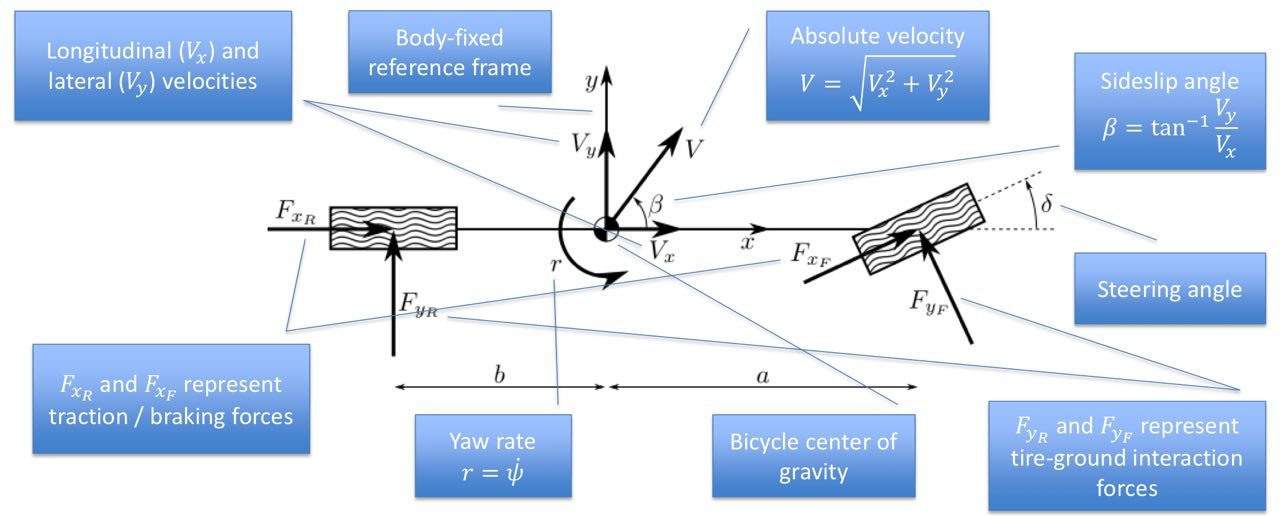
\includegraphics[scale=0.3]{dynamic_model}
	\caption{dynamic model with main parameters and variables}
	\label{fig:dynamic_model}
\end{figure}

\subsection{Configuration}

\begin{center}
	\begin{tabularx}{\textwidth}{
			| >{\raggedright\arraybackslash}X
			| >{\arraybackslash}X |
		}
		\hline
		\multicolumn{2}{|c|}{\textbf{Input values}} \\
		\hline
		$Vp_x$ & Point velocity x \\
		\hline
		$Vp_y$ & Point velocity y \\
		\hline
		$\psi$ & Yaw\footnote{In the System Scheme, this is represented by $\theta_{out}$} \\
		\hline
		$\dot{\psi}$ & Yaw rate\footnote{In the System Scheme, this is \textbf{not} represented (as we have used, for tests, only the kinematic model)} \\
		\hline
	\end{tabularx}
	
	\vspace{0.5cm}
	
	\begin{tabularx}{\textwidth}{
			| >{\raggedright\arraybackslash}X
			| >{\arraybackslash}X |
		}
		\hline
		\multicolumn{2}{|c|}{\textbf{Model parameters}} \\
		\hline
		$C_f$, $C_r$ & Viscuous friction coefficients \\
		\hline
		a, b & Distance between wheels center and Center of Gravity \\		
		\hline
		$M$ & Vehicle mass \\
		\hline
		$\epsilon$ & Distance between Center of Gravity and a point $P$, along the velocity vector. Linearization is done around point P. This parameter should be chosen empirically \\
		\hline
	\end{tabularx}
	
	\vspace{0.5cm}
	
	\begin{tabularx}{\textwidth}{
			| >{\raggedright\arraybackslash}X
			| >{\arraybackslash}X |
		}
		\hline
		\multicolumn{2}{|c|}{\textbf{Intermediate computed values}} \\
		\hline
		$\beta$ & Sideslip angle: $\tan^{-1}\left(\frac{Vp_y}{Vp_x}\right)$ \\
		\hline
	\end{tabularx}
	
	\vspace{0.5cm}
	
	\begin{tabularx}{\textwidth}{
			| >{\raggedright\arraybackslash}X
			| >{\arraybackslash}X |
		}
		\hline
		\multicolumn{2}{|c|}{\textbf{Output values}} \\
		\hline
		$V$ & Point absolute velocity \\
		\hline
		$\delta$ & Steering angle \\
		\hline
		$\omega$ & Steering speed \\
		\hline
	\end{tabularx}
\end{center}

\subsection{Launch}

There is a lunch file which \textbf{should be used to execute the node}. This contains also information about debugging level and loads configuration file.

\subsection{Node car\_dyn\_linearizer}

\[
\beta = \tan^{-1}\left(\frac{Vp_y}{Vp_x}\right)
\]
\[
\delta = \frac{MV}{C_f}\omega + \frac{C_f + C_r}{C_f}\beta - \frac{bC_r - aC_f}{C_f}\frac{\dot{\psi}}{V}
\]
\[
\begin{bmatrix}
	V \\
	\omega
\end{bmatrix}
=
\begin{bmatrix}
	\cos(\beta + \psi) & \sin(\beta + \omega) \\
	-\frac{\sin(\beta + \psi)}{\epsilon} & \frac{\cos(\beta + \psi)}{\epsilon} \\
\end{bmatrix}
\begin{bmatrix}
	Vp_x \\
	Vp_y
\end{bmatrix}
\]